\documentclass{article}
\usepackage{fasy-hw}
\usepackage{amssymb}

%% UPDATE these variables:
\renewcommand{\hwnum}{2}
\title{Discrete Structures, Homework 1}
\author {Robert Marsh (JamesBean)}
\collab{n/a}
\date{due: 5 February 2021}

\begin{document}

\maketitle

This homework assignment should be
submitted as a single PDF file both to D2L and to Gradescope.

General homework expectations:
\begin{itemize}
    \item Homework should be typeset using LaTex.
    \item Answers should be in complete sentences and proofread.
    \item You will not plagiarize.  \item List collaborators at the start of each question using the \texttt{collab} command.
    \item Put your answers where the \texttt{todo} command currently is (and
        remove the \texttt{todo}, but not the word \texttt{Answer}).
\end{itemize}

% ============================================
% ============================================
\collab{n/a} \nextprob{Everyday Mathematical Arguments}
% ============================================
% ============================================
Your sister and you decided to partner on a car washing endeavor, where you
charge cars $\$10$ for a car wash and to split the earnings.  Since you are
doing this at your parents house and they had extra soap, sponges, and a hose
available, there are no costs to you.  At the end of the first day, you have
earned $\$45$ and she had only earned $\$10$. She claimed that you did not pay
her the full payment she deserved. Her argument was: ``If we wash a car, you
earn $\$5$ and I earn $\$5$.  If you earned $\$45$, then we washed nine cars.  If
we wash nine cars, I have earned $\$45$.  I have earned $\$10$; therefore, you
did not give me all of the money that I earned.''  Now, she has not yet taken
Prof.~Fasy's Discrete Structures class, so she does not see the fallacy in her
argument. First, explain which statement that she made that she could not
correctly conclude and explain why.  Second, counter her argument, using
everyday English. The last sentence of your argument should be ``Therefore, I
earned $\$45$ and you earned $\$10$. Third, write this counter argument using
logic statements by first listing the logic statements then writing the argument
mathematically.  Be sure to explain which arguments from Table 2.3.1 that you
are using.

\paragraph{Answer}

Dear sister, you have made the common mistake of the converse error fallacy. You cannot correctly conclude that we washed 9 cars solely based on me earning $\$45$, because it is not necessarily true. I could have earned my $\$45$ from tips or doing other work, not just from washing cars in our car wash. I earned extra money from doing side jobs, not from washing cars. Therefore, I earned $\$45$ and you earned $\$10$.

Consider the following statements:
\begin{enumerate}
    \item p = ``you earned $\$45$''
    \item q = ``we washed $9$ cars''
\end{enumerate}

Using these statements, my argument follows the form of Modus Tollens:

\begin{enumerate}
    \item If we washed 9 cars, you earn $\$45$.
    \item If you earned $\$10$, then we did not wash 9 cars.
    \item Therefore, you did not earn $\$45$.
\end{enumerate}

or 

\begin{enumerate}
    \item $p\implies q$
    \item $\sum q$
    \item $\therefore$ $\sim p$
\end{enumerate}
% ============================================
% ============================================
\collab{\todo{}}
\nextprob{Existential Statements}
% ============================================
% ============================================

Are the following statements true or not true?    Prove or disprove.

\begin{enumerate}

    \item All even integers are equal to an odd integer plus one.

        \paragraph{Answer}
        \todo{be sure to write this in if/then format first.  Then, prove or
        disprove.}

    \item All horses are the same color.

        \paragraph{Answer}
        \todo{be sure to write this in if/then format first.  Then, prove or
        disprove.}

\end{enumerate}


% ============================================
% ============================================
\collab{\todo{}}
\nextprob{Division into Cases}
% ============================================
% ============================================

When working at Lockheed Martin, I was invited to play Texas
Hold'em\footnote{For rules, see
here:\url{https://www.pokernews.com/poker-rules/texas-holdem.htm}} at my
colleague's house.  I play with the following rules:
\begin{itemize}
    \item Never fold before the flop.
    \item Never increase the bet.
    \item If it is possible that my hand is \emph{three of a kind} or better,
        match the bet.  Otherwise, fold.
\end{itemize}
My current hand is the jack of hearts and the 10 of diamonds, and the flop is 10
of hearts, 3 of clubs, and king of hearts.

\begin{enumerate}

    \item What are the cases that could occur for the Turn card?  What is the
        outcome (match or fold) for these different cases? (Note: rather than
        listing every possible card, try to categorize the cards into as few
        classes as possible).

    \paragraph{Answer}
    \todo{your answer here.}

    \item Suppose that the Turn card is the jack of clubs.
        What are the cases that could occur for the River card, and what is the
        outcome (match or fold) for these different cases?  (Again, try to
        describe this in as few cases as possible).

    \paragraph{Answer}
    \todo{your answer here.}

\end{enumerate}


% ============================================
% ============================================
\collab{\todo{}}
\nextprob{Bipartite Graphs}
% ============================================
% ============================================

Exercise Set 4.9, Question 23.

\paragraph{Answer}

\begin{figure}[h]
    \centering
    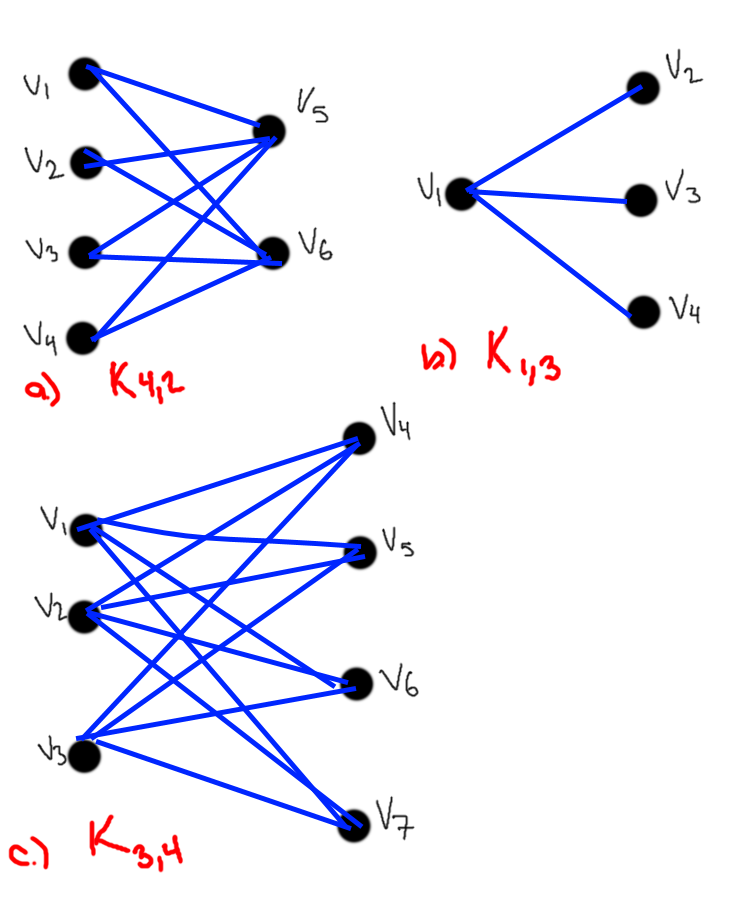
\includegraphics[width=3.5in]{exercise4923}
    \caption{Exercise Set 4.9, Question 23. Part A,B,C.}\label{fig:ex4923}
\end{figure}

\begin{itemize}
    \item [d.] $K_{m,n}$ has $n$ vertices of degree $m$, and $m$ vertices of degree $n$. This is because each member of $n$ has $m$ vertices because it is connected to every $m$, and there are $n$ number of vertices with this property.
    \item [e.] The total degree of $K_{m,n}$ is $2mn$.
    \item [f.] The number of edges of $K_{m,n}$ is $mn$, because it is the total degree of $m$ (or $n$). Each $m$ is connected to each $n$ once and to nothing else (no $(m,m)$ edges), so the total degree of $m$ is equivalent to the number of edges.
\end{itemize}


% ============================================
% ============================================
\collab{\todo{}}
\nextprob{Four Color Theorem}
% ============================================
% ============================================

Read Chapter 1 of \emph{Four Colors Suffice} and answer the following questions:

\begin{enumerate}

    \item Consider the map of the continental US on Page 5.  Why can we color
        Utah and New Mexico the same color, even though the two states touch at
        a point?

        \paragraph{Answer}
        This is allowed because it is a formally agreed upon rule for this problem. Were corner-touching regions required to be different colors, then people could create maps like pie charts, that require up to an infinite number of colors which ruins the whole problem.

    \item Again, looking at the map of the continental US on Page 5, explain why
        Michigan does not satisfy the conditions for the four color theorem.

        \paragraph{Answer}
        Because it is in two pieces - the four color theorem requires that "each country must be in one piece".

    \item Explain why we an omit the states of Hawaii and Alaska in order to
        construct a four-coloring of the states in the USA.

        \paragraph{Answer}
        \todo{your answer here.}

    \item Is the following statement TRUE or FALSE?  Explain. Four colors are
        necessary to color all maps.

        \paragraph{Answer}
        \todo{your answer here.}

    \item Explain one application of the four color theorem that does not
        involve coloring geographic maps.

        \paragraph{Answer}
        \todo{your answer here.}

    \item (Extra Credit). Provide a four-coloring of the McGregor April Fool's
        Hoax on Page 11.

        \paragraph{Answer}
        \todo{Your answer here; should include a figure}

\end{enumerate}

% ============================================
% ============================================
\collab{\todo{}}
\nextprob{Fred Brooks}
% ============================================
% ============================================

Write a short (1-2 paragraph) biography of Fred Brooks.  He wrote the book
entitled \emph{The Mythical Man Month}~\cite{brooks-manmonth}.  In your
biography, explain what the title of this book means.
\textbf{In your own words}, describe who they are and why they are important in
the history of computer science.  If you use external resources, please provide
proper citations. If you do not use external sources, please write ``I did not
use any sources to write this biography'' as the last sentence of the
biography.

\paragraph{Answer}

\todo{your answer goes between these lines}

%% ... the bibliography
\newpage
\bibliographystyle{acm}
\bibliography{biblio}



\end{document}

